\documentclass[10pt]{article}
\label{articlepackage}


\usepackage{soul}
%\usepackage{hyperref}
\usepackage{multicol}

\usepackage{setspace}
%\doublespacing

\usepackage[T1]{fontenc}
\usepackage{ifthen}


\usepackage{bm}
\usepackage{bibentry}
\usepackage{subcaption}

\usepackage{amsmath}
\numberwithin{equation}{section}
\numberwithin{figure}{section}
\numberwithin{table}{section}
\numberwithin{footnote}{section}
\usepackage{mathtools}
\usepackage[inline]{enumitem}
\usepackage{booktabs}
%\usepackage[usenames,dvipsnames,pdftex]{xcolor}
\usepackage{tikz}
\usetikzlibrary{backgrounds,shapes,arrows,positioning,calc,snakes,fit}
\usepgflibrary{decorations.markings}



% \setcounter{section}{-1}

\usepackage{graphicx} % standard package
\usepackage{amsmath} % standard package
\DeclareMathOperator{\sech}{sech}
\newcommand*\diff{\mathop{}\!\mathrm{d}}
\newcommand{\txtd}{\textrm{d}}
\usepackage{amssymb} % useful for double backed letter functions
%%%%%%%%%%%%%%%%%%%%%%%%%%%%%%%%%%%%
\usepackage{amsthm} % used to define theorem objects with command \begin{theorem} etc.
\newtheorem{theorem}{Theorem}[section]
\newtheorem{example}{Example}[subsection]
\newtheorem*{definition}{Definition}
%%%%%%%%%%%%%%%%%%%%%%%%%%%%%%%%%%%%
\newcommand{\eprint}[1]{\href{http://arxiv.org/abs/#1}{#1}}
\usepackage[sort&compress]{natbib}
\bibliographystyle{apsrev} % bibliography package and style
\renewcommand{\bibfont}{\small}
\renewcommand{\citenumfont}[1]{\textbf{#1}}
\renewcommand{\bibnumfmt}[1]{[\color{darkblue}\textbf{#1}\color{black}]}
%%%%%%%%%%%%%%%%%%%%%%%%%%%%%%%%%%%%
\usepackage{listings} % code listing and options
\usepackage{color}
%New colors defined below
\definecolor{codegreen}{rgb}{0,0.6,0}
\definecolor{codegray}{rgb}{0.5,0.5,0.5}
\definecolor{codepurple}{rgb}{0.58,0,0.82}
\definecolor{backcolour}{rgb}{0.95,0.95,0.92}
%Code listing style named "mystyle"
\lstdefinestyle{mystyle}{
  backgroundcolor=\color{backcolour},   commentstyle=\color{codegreen},
  keywordstyle=\color{magenta},
  numberstyle=\tiny\color{codegray},
  stringstyle=\color{codepurple},
  basicstyle=\footnotesize,
  breakatwhitespace=false,
  breaklines=true,
  captionpos=b,
  keepspaces=false,
  numbers=right,
  numbersep=4pt,
  showspaces=false,
  showstringspaces=false,
  showtabs=false,
  tabsize=2
}
\lstset{style=mystyle}

\usepackage[flushmargin, hang]{footmisc}
  \addtolength{\footnotesep}{1mm}
  \setlength{\footnotemargin}{1em}
  \renewcommand{\thefootnote}{\textbf{\arabic{footnote}}}
  \renewcommand\footnoterule{{\hrule height 0.2pt}}

\captionsetup[figure]{labelsep=quad, labelfont=bf, textfont=it, width=0.8\linewidth}


\usepackage{sectsty}
\sectionfont{\color{darkblue}\centering \large \textsc}
\subsectionfont{\color{darkblue}\centering \normalsize \textit}
\subsubsectionfont{\color{darkblue}\centering \small \textit}
\renewcommand\thesection{\arabic{section}}
\renewcommand\thesubsection{\arabic{section}.\arabic{subsection}}
\renewcommand\thefigure{\arabic{section}.\arabic{figure}}
\renewcommand\theequation{{\color{SAEblue}\arabic{section}.\arabic{equation}}}
\usepackage{color}
\definecolor{SAEblue}{rgb}{0, .62, .91}
\definecolor{linkgreen}{RGB}{11, 102, 35}
\definecolor{darkblue}{rgb}{.11, .102, .35}

\usepackage[colorlinks]{hyperref}
\hypersetup{colorlinks=true, urlcolor=linkgreen, citecolor=linkgreen, runcolor=black, menucolor=black, filecolor=black, anchorcolor=black, linkcolor=black}
\theoremstyle{definition}


\theoremstyle{definition}

\renewcommand\vec{\mathbf}
\newcommand{\normord}[1]{\raisebox{0.5pt}{:}\,#1\,\raisebox{0.5pt}{:}}
\newcommand{\dagg}{^{\dagger}}
\newcommand{\pr}{^{\prime}}
\newcommand{\nhat}{\hat{\bm{n}}}
\newcommand{\hamilt}{\mathcal{H}}
\newcommand{\mA}{\mathcal{A}}
\newcommand{\mW}{\mathcal{W}}
\newcommand{\mN}{\mathcal{N}}
\newcommand{\mD}{\mathcal{D}}
\newcommand{\mS}{\mathcal{S}}
\newcommand{\mL}{\mathcal{L}}
\newcommand{\mC}{\mathcal{C}}
\newcommand{\mO}{\mathcal{O}}
\newcommand{\mM}{\mathcal{M}}
\newcommand{\mT}{\mathcal{T}}
\newcommand{\mZ}{\mathcal{Z}}
\newcommand{\mR}{\mathcal{R}}
\newcommand{\II}{\mathbb{I}}
\newcommand{\RR}{\mathbb{R}}
\newcommand{\ZZ}{\mathbb{Z}}
\newcommand{\CC}{\mathbb{C}}
\newcommand{\FF}{\mathbb{F}}
\newcommand{\lie}[1]{\mathcal{L}\left(#1\right)}
\newcommand{\set}[1]{\left\{#1\right\}}
\newcommand{\SO}[1]{\textrm{SO}\left(#1\right)}
\newcommand{\SU}[1]{\textrm{SU}\left(#1\right)}
\newcommand{\Orth}[1]{\textrm{O}\left(#1\right)}
\newcommand{\Uni}[1]{\textrm{U}\left(#1\right)}
\newcommand{\paraskip}{\vspace{10pt}}
\newcommand{\del}{\partial}
\newcommand{\TeG}{\mathcal{T}_e(\mathscr{G})}
\newcommand{\TpM}{\mathcal{T}_p(\mathcal{M})}
\newcommand{\TpMs}{\mathcal{T}^{\star}_p(\mathcal{M})}
\newcommand{\etamn}[1]{\eta#1{\mu \nu}}
\newcommand{\upd}[1]{\text{d}#1 \,}
\newcommand{\ud}{\text{d}}
\newcommand{\group}{\mathscr{G}}
\newcommand{\alge}{\mathfrak{g}}
\newcommand{\twobytwo}[4]{\begin{pmatrix}#1&#2 \\ #3&#4 \end{pmatrix}}
\newcommand{\thrbythr}[3]{\begin{pmatrix}#1 \\ #2 \\ #3\end{pmatrix}}
\newcount\colveccount
\newcommand*\colvec[1]{
        \global\colveccount#1
        \begin{pmatrix}
        \colvecnext
}
\def\colvecnext#1{
        #1
        \global\advance\colveccount-1
        \ifnum\colveccount>0
                \\
                \expandafter\colvecnext
        \else
                \end{pmatrix}
        \fi
}

\newenvironment{Figure}
  {\par\medskip\noindent\minipage{\linewidth}}
  {\endminipage\par\medskip}

\newcommand{\Abs}[1]{\left| #1 \right|}
\newcommand{\tr}{\text{Tr}}

\renewcommand\labelitemi{\raisebox{0.25ex}{\tiny$\bullet$}}
\setenumerate{label=\color{SAEblue}{\textbf{\arabic*}}\color{black})}

\usepackage[labelfont=bf]{caption}
\usepackage[margin=0.8in]{geometry}
\usepackage{fancyhdr}
\pagestyle{fancy}
\lhead{\small\textsc{Atmospheric Flux}}
\chead{}
\rhead{}
\lfoot{}
\cfoot{\textit{\thepage}}
\rfoot{}

\newcommand{\plotdir}[1]{/mnt/james/allMyStuff/BoostedDM/Python/plots/#1}
%\renewcommand{\plotdir}[1]{/Users/james/allMyStuff/BoostedDM/Python/plots/#1}
\renewcommand*{\thefootnote}{\fnsymbol{footnote}}
\setcounter{footnote}{1}

\begin{document}
\hrule
\vspace{1pt}
\hrule
\begin{center}
\large\textsc{\color{darkblue}\textbf{Calculating the Atmospheric Flux}}
\vspace{5pt}

\footnotesize\textit{\textbf{J.B.G. Alvey}, Theoretical Particle Physics and Cosmology, King's College London\footnote{\href{mailto:james.alvey@kcl.ac.uk}{james.alvey@kcl.ac.uk}}}
\end{center}
\begin{abstract}
\noindent Set of notes discussing the calculations involved in obtaining the atmospheric dark matter flux $\textrm{d}\phi_\chi/\textrm{d}T_\chi$ due to $pN \rightarrow \pi_0 \rightarrow \gamma\chi\chi$ interactions in the Earth's atmosphere.
\end{abstract}
\hrule
\tableofcontents
\vspace{5pt}
\hrule
\vspace{1pt}
\hrule
\vspace{10pt}
\renewcommand{\thefootnote}{\tiny\textbf{\arabic{section}.\arabic{footnote}}}
%\begin{multicols*}{2}
\section{Suppression of the Incident Proton Flux}
If we assume there is an initial proton flux, as measured for example by the AMS experiment, at the top of the atmosphere, then interactions with nitrogen molecules in the air will lead to a suppression at heights below this initial value. This will depend on the total inelastic cross section between the protons and the nitrogen molecules. The numerical value of this cross section, $\sigma_{pN}^{\textrm{\small inel}}$ is plotted in Figure \ref{fig:pnsigma}. We see from this that the cross section is approximately constant across the energy range where the AMS flux is parameterised (approximately $10^1 - 10^3 \, \textrm{GeV}$). As such, in what follows, we take th simplifying assumption that $\sigma_{pN}^{\textrm{\small inel}}$ is constant, with a value of $255 \, \textrm{mb}$. Now, denote the proton flux as a function of proton energy and height as $\textrm{d}\phi_p/\textrm{d}T_p(T_p, h)$. Evaluated at $h_{\textrm{\small max}} \simeq 180 \, \textrm{km}$, this is equal to the AMS flux discussed above. Letting the number density of nitrogen molecules in the atmosphere be $n_N(h)$, which is shown in Figure \ref{fig:airdensity}, the flux satisfies;
\begin{center}
  \begin{figure}[h]
    \centering
    \begin{subfigure}[t]{0.3\textwidth}
        \centering
        \includegraphics[width=\textwidth]{\plotdir{pNsigma.pdf}}
        \caption{The total $pN$ cross section as a function of incident proton energy.}
        \label{fig:pnsigma}
    \end{subfigure}%
    \hfill
    \begin{subfigure}[t]{0.3\textwidth}
        \centering
        \includegraphics[width=\textwidth]{\plotdir{air_density.pdf}}
        \caption{The number density of nitrogen molecules in the Earth's atmosphere as a function of height.}
        \label{fig:airdensity}
    \end{subfigure}
    \hfill
    \begin{subfigure}[t]{0.3\textwidth}
        \centering
        \includegraphics[width=\textwidth]{\plotdir{suppression.pdf}}
        \caption{The suppression function $Y(h)$ as a function of $h$.}
        \label{fig:supp}
    \end{subfigure}
    \caption{Plots of the $pN$ cross section and the air density.}
    \label{fig:pnair}
  \end{figure}
\end{center}
\begin{equation}
  \label{eq:sup}
  \frac{\ud}{\ud h}\frac{\ud \phi_p(T_p, h)}{\ud T_p} = \sigma_{pN}^{\textrm{\small inel}}n_N(h)\frac{\ud \phi_p(T_p, h)}{\ud T_p}
\end{equation}
With the simplifying assumption regarding the cross section we see that this is now separable. If we let;
\begin{equation}
  \frac{\ud \phi_p(T_p, h)}{\ud T_p} := Y(h)\frac{\ud\phi_p(T_p, h_{\textrm{\small max}})}{\ud T_p}
\end{equation}
In other words, we introduce a suppression factor $Y(h)$ normalised such that $Y(h_{\textrm{\small max}} = 180\,\textrm{km}) = 1$. Substituting this into \eqref{eq:sup}, we find the following equation for $Y(h)$,
\begin{equation}
  \frac{\ud Y(h)}{\ud h} = \sigma_{pN}^{\textrm{\small inel}} n_N(h) Y(h)
\end{equation}
Integrating and using the initial conditions on $Y(h)$ we find the solution;
\begin{equation}
  Y(h) = \exp\left(-\sigma_{pN}^{\textrm{\small inel}}\int_{h}^{h_{\textrm{\small max}}}{\upd{\tilde{h}} n_N(\tilde{h})}\right)
\end{equation}
We can integrate this numerically using the parameterisation for the number density, the results are shown in Figure \ref{fig:supp}. We note in particular that it is approximately constant above $h = 20 \, \textrm{km}$, below which is decreases rapidly. \textbf{Something to consider is whether the function} $Y(h)$ \textbf{should depend on angle} $\theta$.
\section{The Resultant Dark Matter Flux}
Now we have an expression for the attenuation of the proton flux as a function of height, we need to calculate the dark matter flux $\ud \phi_\chi/\ud T_\chi$. If we let the radius of the Earth be $R_E = 6378.1 \, \textrm{km}$, then the differential flux can be calculated via;
\begin{multline}
  \frac{\ud \phi_\chi}{\ud T_\chi} = \int_{0}^{H}{(R_E + h)^2\upd{h}\int_0^{2\pi}{\upd{\phi} \int_{-1}^{+1}{\upd{\cos\theta}\frac{n_N(h)Y(h)}{2\pi \ell(R_E + h, \theta)^2}}}\times \int_{T_p^{\textrm{\tiny min}}}^{T_p^{\textrm{\tiny max}}}}{\upd{T_p} \sigma_{pN\rightarrow \chi\chi}(T_p)f(T_p, T_\chi)\frac{\ud \phi_p(T_p, h_{\textrm{\small max}})}{\ud T_p}}
\end{multline}
There are a couple of things to notice about this formula. Firstly, the geometry is shown in Figure \ref{fig:geometry}, with the angles $\theta$ and $\phi$ as illustrated. It has been assumed that the Earth is transparent to dark matter in this case. With these definitions, the function $\ell(r, \theta)$ is given by;
\begin{equation}
  \ell^2(r, \theta) = 2 R_E r (1 - \cos\theta) + (r - R_E)^2
\end{equation}
Secondly, we note that the simplification that the $pN$ cross section is independent of energy ensures that the prefactor before the multiplication sign is just a constant geometrical factor, which we denote $F_p$. This means that the Monte Carlo techniques used to evaluate the second integral can be performed independently. From a notational perspective, $f(T_p, T_\chi)$ accounts for the multiplicity of the dark matter particles produced at each energy $T_\chi$ for a given proton energy $T_p$. It should have units of inverse energy. Finally, $H$ is some reference height up to which the integration is performed which should be determined.
\subsection{The Geometrical Factor}
We evaluate the geometrical factor in the case that $Y(h)$ does not depend on the angle. In this case, the integral becomes;
\begin{align*}
  F_g(h_1, h_2) &= \int_{h_1}^{h_2}{\upd{h} (R_E + h)^2 \int_{0}^{2\pi}{\upd{\phi} \int_{-1}^{+1}{\upd{\cos\theta}n_N(h)Y(h)\frac{1}{2\pi \ell^2(R_E + h, \theta)}  } } } \\
  &= 2\pi\int_{h_1}^{h_2}{\upd{h} (R_E + h)^2 \int_{-1}^{+1}{\upd{\cos\theta}n_N(h)Y(h)\frac{1}{2\pi \left(2R_E (R_E + h)(1 - \cos\theta) + h^2\right)}  } } \\
  &= \int_{h_1}^{h_2}{\upd{h} (R_E + h)^2 n_N(h)Y(h) \int_{-1}^{+1}{\upd{\cos\theta}\frac{1}{ \left(2R_E (R_E + h)(1 - \cos\theta) + h^2\right)}  } }
\end{align*}
Using the fact that $2R_E(R_E + h) + h^2 \geq 2R_E(R_E + h) > 0$, we can do the angular integration analytically to obtain;
\begin{equation}
  F_g(h_1, h_2) = \int_{h_1}^{h_2}{\upd{h} \frac{R_E + h}{2R_E} n_N(h)Y(h) \log\left(\frac{4R_E(R_E + h) + h^2}{h^2}\right)}
\end{equation}
The results of doing this integral and the corresponding atmospheric flux are given in Figure \ref{fig:atmosdmflux}.
\begin{center}
  \begin{figure}[h]
    \centering
    \includegraphics[width=0.7\textwidth]{\plotdir{atmos_dm_flux_pospelov.pdf}}
    \caption{The resulting dark matter flux, not accounting for any attenuation after it is produced.}
    \label{fig:atmosdmflux}
  \end{figure}
\end{center}
\section{Full Derivation including Attenuation}
Ultimately the goal is to calculate the dark matter flux a depth $h_d$ below the surface of the Earth, where the detector is located. For Xenon 1T, this depth is approximately $6\,\textrm{km}$. To do so, we first compute the flux of dark matter particles produced $\textrm{cm}^{-3}\,\textrm{s}^{-1}\,\textrm{GeV}^{-1}$ at a position $(h, \theta, \phi)$, as labelled in Figure \ref{fig:dmatt}. Furthermore, we assume that the flux produced at this point recieves an attentuation due to nucleon interactions given by $Y_d(h, \theta, \phi)$. In other words, there is a position dependent attenuation that depends on the line of sight density to the detector. The total dark matter flux at the detector is then an integral over all the possible production points;
\begin{equation}
  \frac{\ud \phi^{\textrm{\tiny det}}_\chi}{\ud T_\chi}[\textrm{cm}^{-2}\,\textrm{s}^{-1}\,\textrm{GeV}^{-1}] = \int_{0}^{h_{\textrm{\tiny max}}}{\upd{h} (R_E + h)^2 \int_{0}^{2\pi}{\upd{\phi} \int_{-1}^{+1}{\upd{\cos\theta} \frac{1}{\ell^2_d(h, \theta)} Y_d(h, \theta, \phi) \frac{\ud \phi_\chi}{\ud\cos\theta \, \ud \phi \, \ud h \, \ud T_\chi}  }  }  }
\end{equation}
where $\ud \phi_\chi/\ud\cos\theta \,\ud \phi\, \ud h \,\ud T_\chi \,[\textrm{cm}^{-3}\,\textrm{s}^{-1}\,\textrm{sr}^{-1}\,\textrm{GeV}^{-1}]$ is the flux of dark matter particles produced at a position $(h, \theta, \phi)$. Furthermore, $l_d(h, \theta)$ denotes the line of sight distance between the production point and the detector.  It is given by;
\begin{equation}
  \ell^2_d(h, \theta) = (R_E + h)^2 + (R_E - h_d)^2 - 2(R_E + h)(R_E - h_d)\cos\theta
\end{equation}
\begin{center}
  \begin{figure}[h]
    \centering
    \includegraphics[width=0.4\textwidth]{\plotdir{nE.pdf}}
    \caption{The number density within the Earth assuming the average mass per nucleon is $11.8871 m_p$.}
    \label{fig:patt2}
  \end{figure}
\end{center}
\subsection{The Supression Factor $Y_d(h, \theta, \phi)$}
If a flux $\ud \phi_\chi/\ud T_\chi$ propagates along a line of sight from $(h, \theta, \phi)$ to the detector, and the cross-section $\sigma_{\chi N}$ is independent of energy, then we should do the following integral,
\begin{equation}
  \label{eq:yd}
  Y_d(h, \theta, \phi) = \exp\left(-\sigma_{\chi N} \int_{\mathcal{C}}{\upd{\ell} n}\right)
\end{equation}
where $n$ is the number density, a plot of which is shown in Figure \ref{fig:nE}. If we parametrise the path as in \ref{fig:dmatt} then the suppression factor is given by;
\begin{center}
  \begin{figure}[h]
    \centering
    \begin{subfigure}[t]{0.45\textwidth}
        \centering
        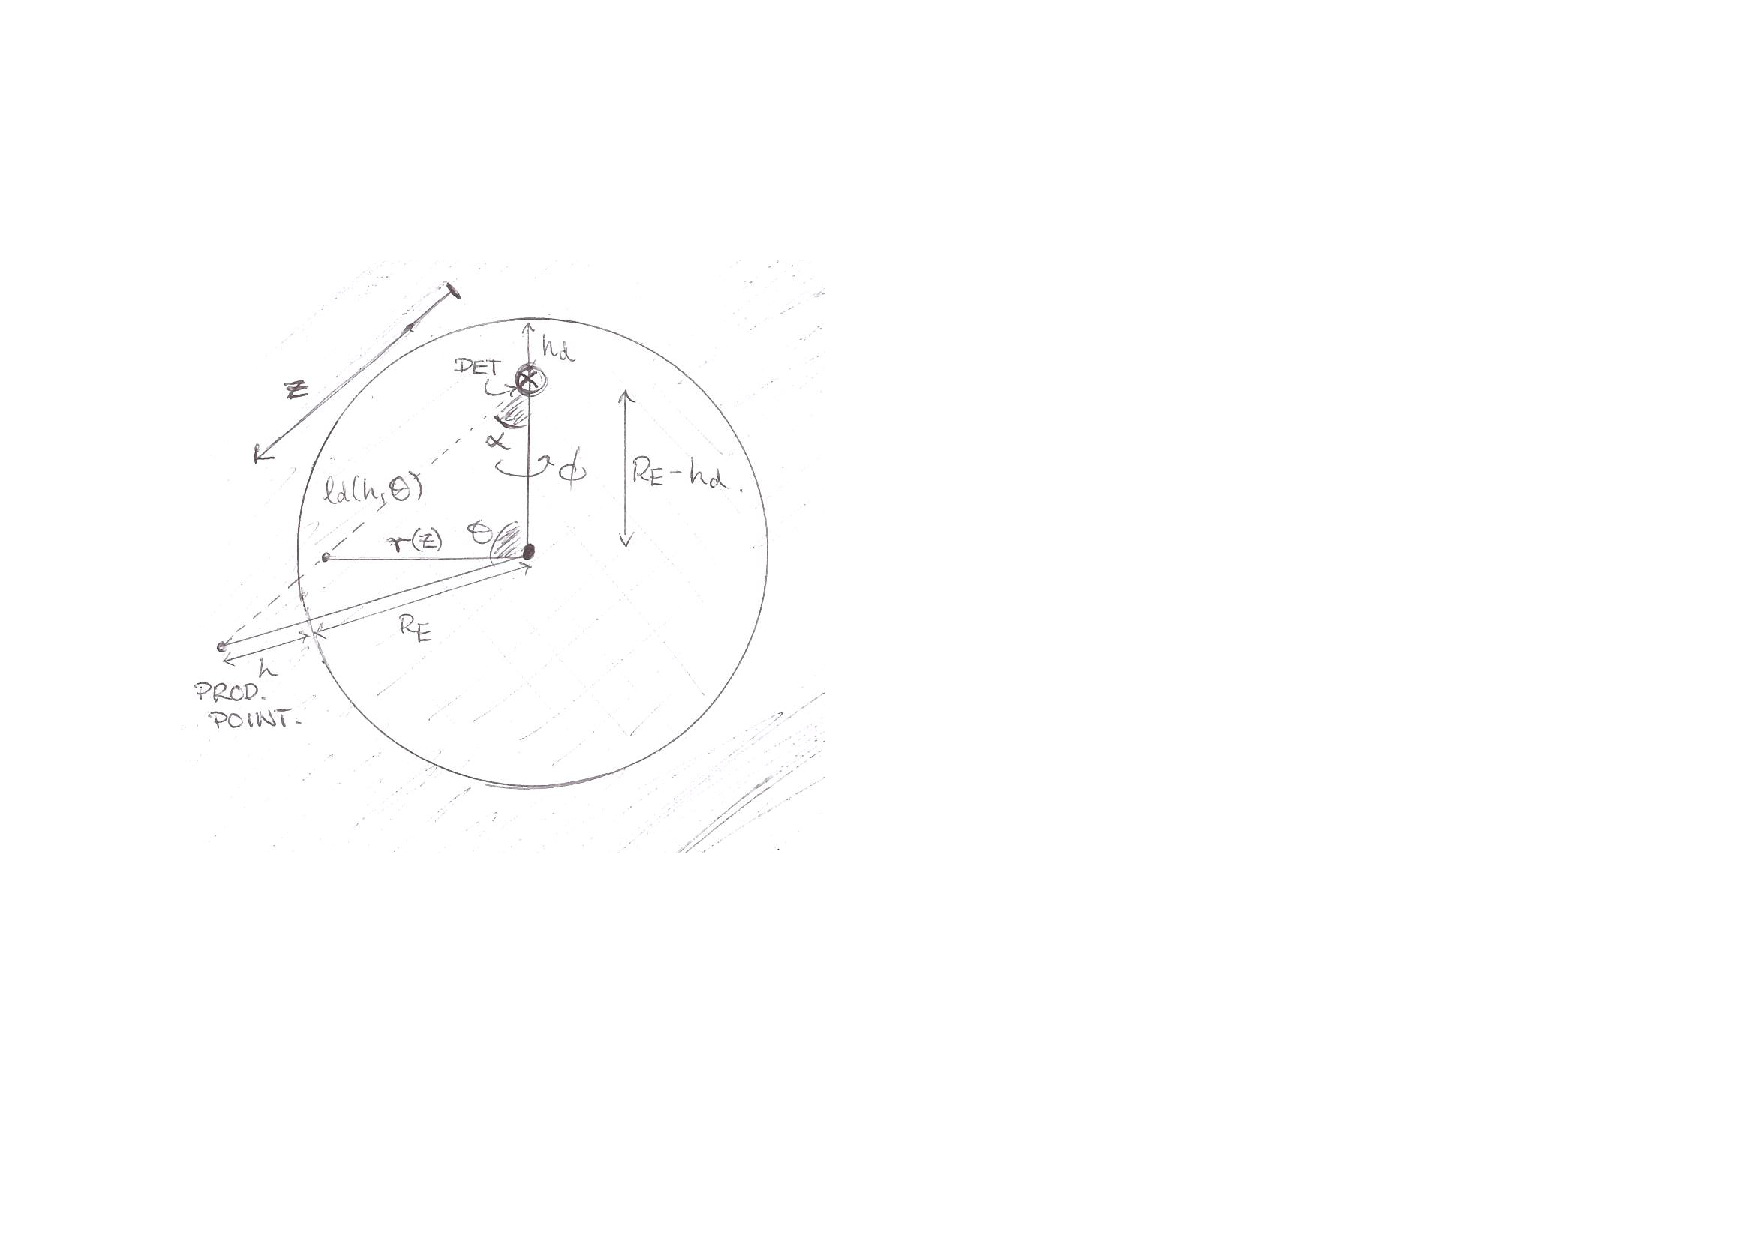
\includegraphics[width=\textwidth]{dmattenuation.pdf}
        \caption{The geometry of the detector location at a depth $h_d$ below the Earth's surface.}
        \label{fig:dmatt}
    \end{subfigure}%
    \hfill
    \begin{subfigure}[t]{0.45\textwidth}
        \centering
        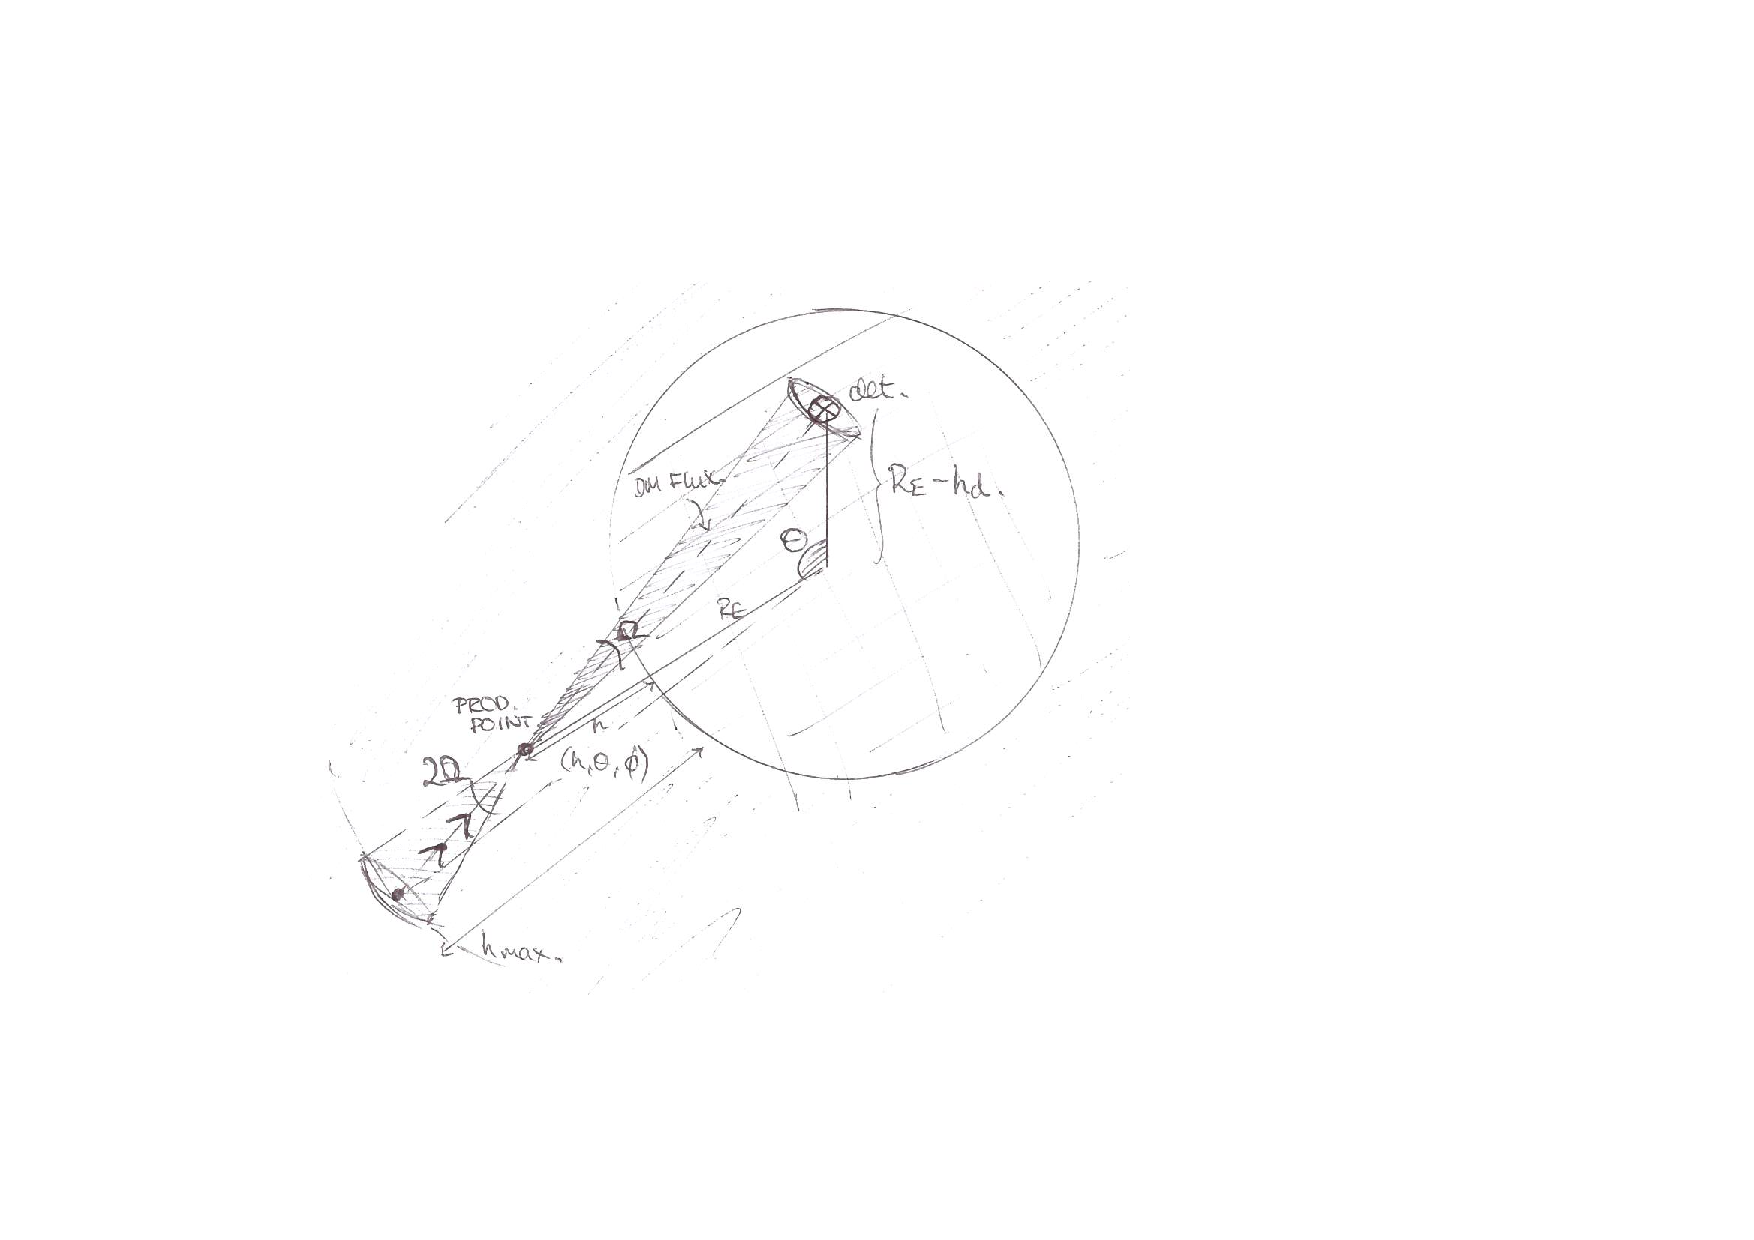
\includegraphics[width=\textwidth]{pattenuation.pdf}
        \caption{The geometry for the proton attenuation as a function of height.}
        \label{fig:patt}
    \end{subfigure}
    \caption{Geometries for the attenuation of the dark matter and the proton fluxes}
    \label{fig:pnair}
  \end{figure}
\end{center}
\begin{equation}
  \label{eq:dmsup}
  Y_d(h, \theta, \phi) = \exp\left(-\sigma_{\chi N} \int_{0}^{\ell_d(h, \theta)}{\upd{z}n\left(r(z) - R_E\right)}\right)
\end{equation}
The choice of radial co-ordinate is in line with our definition of the nitrogen density using $h = 0$ as the surface of the Earth. To find $r(z)$, we use;
\begin{equation}
  \frac{\ell_d(h, \theta)}{\sin\theta} = \frac{R_E + h}{\sin\alpha} \Rightarrow \sin\alpha = \frac{(R_E + h)\sin\theta}{\ell_d(h, \theta)}
\end{equation}
Then we can calculate;
\begin{equation}
  r(z, h, \theta)^2 = (R_E - h_d)^2 + z^2 - \textrm{sign}\left[(R_E - h_d) - (R_E + h)\cos\theta\right]2(R_E - h_d)z\left(1 - \frac{(R_E + h)^2\sin^2\theta}{\ell^2_d(h, \theta)}\right)^{1/2}
\end{equation}
\begin{center}
  \begin{figure}[h]
    \centering
    \begin{subfigure}[t]{0.45\textwidth}
        \centering
        \includegraphics[width=\textwidth]{\plotdir{rexamples.pdf}}
        \caption{The function $r(z, h, \theta)$ illustrating the expected behaviour for different values of $\theta$.}
        \label{fig:rexample}
    \end{subfigure}%
    \hfill
    \begin{subfigure}[t]{0.45\textwidth}
        \centering
        \includegraphics[width=\textwidth]{\plotdir{Ydcontour.pdf}}
        \caption{A contour plot of $Y_d(h, \theta, \sigma_\chi^{\textrm{SI}} = 10^{-32}\,\textrm{cm}^2)$.}
        \label{fig:Ydcontour}
    \end{subfigure}
    \caption{The behaviour of $Y_d(h, \theta, \sigma_\chi^{\textrm{SI}})$ and $r(z, h, \theta)$ as a function of $h$ and $\theta$.}
    \label{fig:Yd}
  \end{figure}
\end{center}
where the $\pm$ arises due to the angle $\alpha$ being acute or obtuse. In the former case, $\cos\alpha$ will be positive, whilst in the latter case it will be negative. This is shown in Figure \ref{fig:rexample}. From this we can also derive the line of sight distance only through the Earth by noticing that this distance is given by $z_{\star}$ where $r(z_\star, h, \theta) = R_E$. There will be two such solutions, one positive, and one negative. We should take the positive one. This satisfies;
\begin{equation}
R_E^2 = (R_E - h_d)^2 + z_\star^2 - \textrm{sign}\left((R_E - h_d) - (R_E + h)\cos\theta\right)\cdot 2(R_E - h_d)z_\star\left(1 - \frac{(R_E + h)^2 \sin^2\theta}{\ell_d^2(h, \theta)}\right)^{1/2}
\end{equation}
Solving for $z_\star$, we find;
\begin{equation}
  z_\star = \frac{1}{2}\left(b(h, \theta) + \sqrt{b^2(h, \theta) + 4\left(R_E^2 - (R_E - h_d)^2\right)}\right)
\end{equation}
where,
\begin{equation}
  b(h, \theta) = \textrm{sign}\left((R_E - h_d) - (R_E + h)\cos\theta\right)\cdot 2(R_E - h_d)\left(1 - \frac{(R_E + h)^2 \sin^2\theta}{\ell_d^2(h, \theta)}\right)^{1/2}
\end{equation}
\begin{center}
  \begin{figure}[h]
    \centering
    \begin{subfigure}[t]{0.45\textwidth}
        \centering
        \includegraphics[width=\textwidth]{\plotdir{zstarexample.pdf}}
        \caption{The function $z_\star(h, \theta)$ illustrating the expected behaviour for different values of $\theta$.}
        \label{fig:zexample}
    \end{subfigure}%
    \hfill
    \begin{subfigure}[t]{0.45\textwidth}
        \centering
        \includegraphics[width=\textwidth]{\plotdir{zstarcontour.pdf}}
        \caption{A contour plot of $Y_d(h, \theta, \sigma_\chi^{\textrm{SI}} = 10^{-32}\,\textrm{cm}^2)$.}
        \label{fig:zstarcontour}
    \end{subfigure}
    \caption{The behaviour of $z_\star(h, \theta)$ as a function of $h$ and $\theta$.}
    \label{fig:zstar}
  \end{figure}
\end{center}
The results are shown in Figure \ref{fig:zstar} for a detector at depth 1.4 km. If we assume a distinction between the core and the mantle, then we also need to calculate how much of this path is within the core, with radius $r_c$. For a given height $h$, the line of sight will intersect the core only if;
\begin{equation}
\theta > \theta_{\star}(h) = \arccos\left(\frac{r_c}{R_E - h_d}\right) + \arccos\left(\frac{r_c}{R_E + h}\right)
\end{equation}
Now, if $\theta$ is indeed larger than this value, then we can calculate the two line of sight distances $z_{\textrm{core}}$ and $z_{\textrm{mantle}}$. This can be done by solving for $z$ when $r(z, h, \theta) = r_c$. For $\theta > \theta_{\star}(h)$ this will give two solutions, the difference of which is $z_{\textrm{core}}$;
\begin{equation}
  z_{\textrm{core}}(h, \theta) = \sqrt{b(h, \theta)^2 - 4\left((R_E - h_d)^2 - r_c^2\right)}
\end{equation}
This can then be used to calculate $z_{\textrm{mantle}}(h, \theta)$. Taking into account the cutoff on $\theta$ due to the finite extent of the core, we find;
\begin{equation}
  z_{\textrm{core}}(h, \theta) = \begin{cases} 0 & \text{if } \theta \leq \theta_{\star}(h) \\ \sqrt{b(h, \theta)^2 - 4\left((R_E - h_d)^2 - r_c^2\right)} & \text{if } \theta > \theta_{\star}(h)\end{cases}, \qquad z_{\textrm{mantle}}(h, \theta) = z_{\star}(h, \theta) - z_{\textrm{core}}(h, \theta)
\end{equation}
We can then substitute these definitions into \eqref{eq:dmsup} to find the suppression factor $Y_d(h, \theta)$. In order to actually calculate this, we need to parametrise the number density of the Earth. We also need to understand what $\sigma_{\chi N}$ represents in \eqref{eq:yd}. From the Pospelov paper, we have the expression;
\begin{equation}
  \sigma_{\chi N} = \sigma_\chi^{\textrm{SI}} A^2 \left(\frac{m_N(m_\chi + m_p)}{m_p(m_\chi + m_N)}\right)^2
\end{equation}
The mass range of dark matter we are interested in means that $m_\chi \ll m_p, m_N$ so we can approximate this by;
\begin{equation}
  \sigma_{\chi N} = \sigma_{\chi}^{\textrm{SI}}A^2
\end{equation}
The number quoted is $A^2 = 165.025$ is a weighted sum of the fractions of elements in the Earth's crust and mantle. A similar weighted average gives a nuclear mass of $11.8871 m_p$. This will be used to convert the density in units $\textrm{g}\,\textrm{cm}^{-3}$ to a number density in units $\textrm{cm}^{-3}$. The results for a cross section of $\sigma_chi^{\textrm{SI}} = 10^{-32}\,\textrm{cm}^2$ are shown in Figure \ref{fig:Ydcontour}.
\subsection{Attenuation of the Proton Flux}
It remains to calculate the factor $\ud \phi_\chi / \ud \cos\theta \, \ud \phi \,\ud h \, \ud T_\chi$. This is given by;
\begin{equation}
  \frac{\ud \phi_\chi (h, \theta, \phi)}{\ud\cos\theta \, \ud \phi \, \ud h} = n_N(h) \int_{T_p^{\textrm{\tiny min}}}^{T_p^{\textrm{\tiny max}}}{\upd{T_p}\frac{1}{\Omega(T_p)}\frac{\ud\phi_p(T_p; h, \theta, \phi)}{\ud T_p}\frac{\ud \sigma_{pN \rightarrow \chi\chi}(T_p)}{\ud T_\chi}}
\end{equation}
where $\Omega(T_p)$ is the opening solid angle for the boosted dark matter pointing towards the detector, as in Figure \ref{fig:patt}. We see that we need to determine the proton flux as a function of $h$ and $\theta$. Note that we are interested only in the proton flux that will lead to dark matter that actually hits the detector. This is in contrast to the expressions in the simplified case, where the opening angle was assumed to be $2\pi$. Now, the flux that leads to dark matter travelling towards the detector can be written as;
\begin{equation}
  \frac{\ud \phi_p(h, \theta)}{\ud T_p} = Y_p(h, \theta)\frac{\ud \phi_p(h_{\textrm{\tiny max}})}{\ud T_p}
\end{equation}
Here, $Y_p(h, \theta)$ denotes the average suppression that accounts for the propagation of protons from all points in the solid angle $2\Omega$ as in Figure \ref{fig:patt}. If we let this region of solid angle be denoted $\mathcal{A}$, then;
\begin{equation}
  Y_p(h, \theta) = \frac{\int_{\mathcal{A}}{\upd{\tilde{\Omega}} \exp\left(-\sigma_{pN}^{\textrm{\tiny inel.}} \int_{\mathcal{C}}{n\,\ud l}\right)   }}{\int_{\mathcal{A}}{\upd{\tilde{\Omega}}}}
\end{equation}
where the line of sight integration along $\mathcal{C}$ depends on the path from the edge of the atmosphere to the point $(h, \theta, \phi)$. For small $\Omega$, this is approximately given by;
\begin{equation}
  Y_p(h, \theta) \simeq \exp\left(-\sigma_{pN}^{\textrm{\tiny inel.}} \int_{\mathcal{C^\star}}{n_N \, \ud l}\right)
\end{equation}
where now $\mathcal{C}^\star$ is the line of sight between the edge of the atmosphere and the detector, through the point $(h, \theta, \phi)$. This is illustrated in Figure \ref{fig:patt2}. With these definitions, we have;
\begin{equation}
    Y_p(h, \theta) = \exp\left(-\sigma_{pN}^{\textrm{\tiny inel.}}\int_{0}^{\ell_p(h, \theta)}{\upd{\tilde{z}}n_N\left(r_p(\tilde{z}) - R_E\right)}\right)
\end{equation}
Now we need to find $\ell_p(h, \theta)$ and $r_p(\tilde{z}, h, \theta)$. We let $\theta_2$ be the angle between the detector, the point $(h, \theta, \phi)$ and the centre of the Earth, and the angle $\alpha_1$ be the one between the centre of the Earth, the point at $h_{\textrm{\tiny max}}$ and the detector. Then we find;
\begin{center}
  \begin{figure}[h]
    \centering
    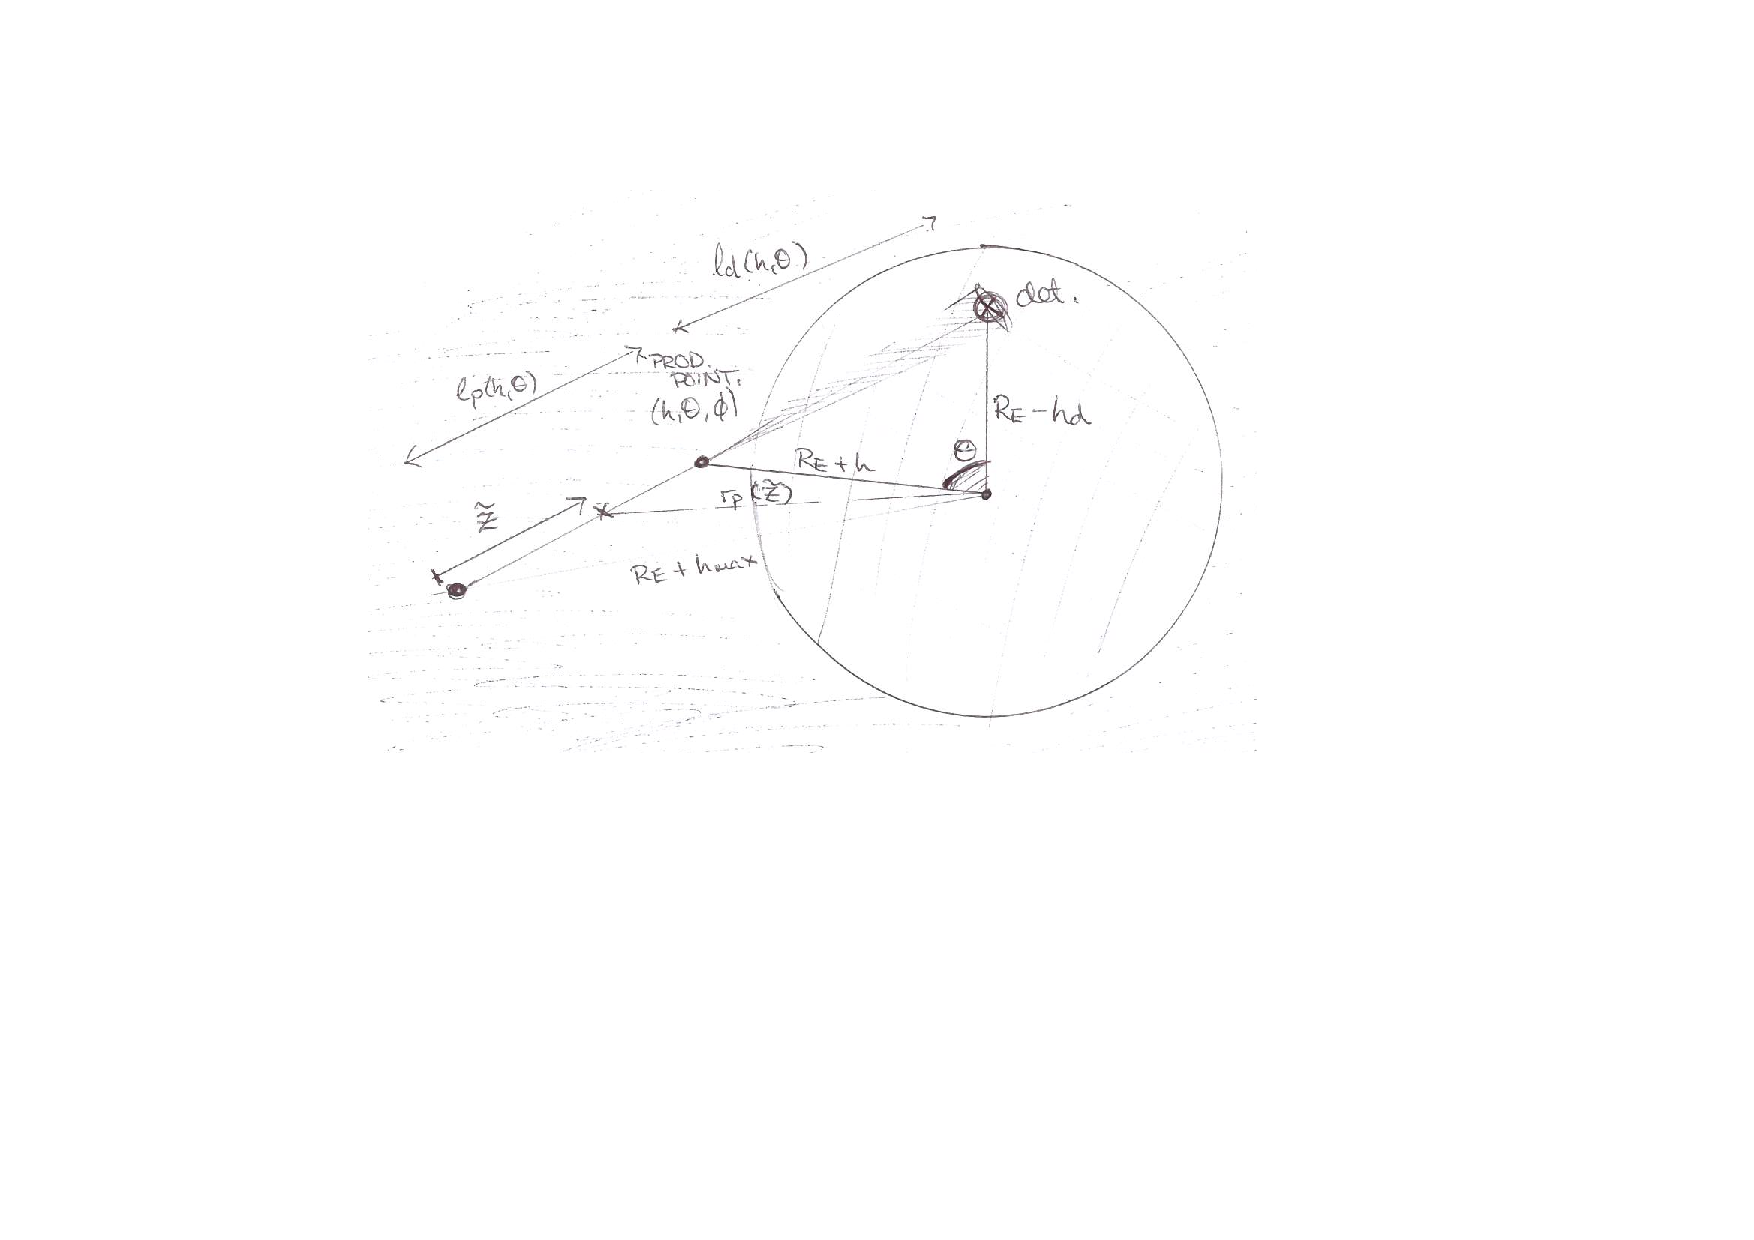
\includegraphics[width=0.6\textwidth]{pattenuation2.pdf}
    \caption{The geometry of the integration over the proton path.}
    \label{fig:patt2}
  \end{figure}
\end{center}
\begin{equation}
  r^2_p(\tilde{z}, h, \theta) = (R_E + h_{\textrm{\tiny max}})^2 + \tilde{z}^2 - 2(R_E + h_{\textrm{\tiny max}})\tilde{z}\cos\alpha_1
\end{equation}
Using the sine rule, we have;
\begin{equation}
    \frac{\ell_d(h, \theta)}{\sin\theta} = \frac{R_E - h_d}{\sin\theta_2} \,\, \Rightarrow \,\, \sin\theta_2 = \frac{(R_E - h_d)\sin\theta}{\ell_d(h, \theta)}
\end{equation}
So,
\begin{equation}
  \frac{R_E + h_{\textrm{\tiny max}}}{\sin(\pi - \theta_2)} = \frac{R_E + h}{\sin\alpha_1} \,\,\Rightarrow\,\, \sin\alpha_1 = -\frac{(R_E + h)(R_E - h_d)\sin\theta}{(R_E + h_{\textrm{\tiny max}})\ell_d(h, \theta)}
\end{equation}
This in turn implies that;
\begin{equation}
  \cos\alpha_1 = \left(1 - \frac{(R_E + h)^2(R_E - h_d)^2\sin^2\theta}{(R_E + h_{\textrm{\tiny max}})^2\ell^2_d(h, \theta)}\right)^{1/2}
\end{equation}
Then we can write down $r_p(\tilde{z}, h, \theta)$ as;
\begin{equation}
  r^2_p(\tilde{z}, h, \theta) = (R_E + h_{\textrm{\tiny max}})^2 + \tilde{z}^2 - 2(R_E + h_{\textrm{\tiny max}})\tilde{z}\left(1 - \frac{(R_E + h)^2(R_E - h_d)^2\sin^2\theta}{(R_E + h_{\textrm{\tiny max}})^2\ell^2_d(h, \theta)}\right)^{1/2}
\end{equation}
Note in this case that we do not have the same issues with positive and negative $\cos\alpha_1$ as one can check that it does not change sign and is initially positive for $\theta = 0$. Now to find $\ell_p(h, \theta)$, we note that $\tilde{z} = R_E + h$ when $r_p(\tilde{z}) = \ell_p(h, \theta)$. So we can solve the quadratic in $\ell_p(h, \theta)$ given by;
\begin{equation}
  (R_E + h)^2 = (R_E + h_{\textrm{\tiny max}})^2 + \ell^2_p(h, \theta) - 2(R_E + h_{\textrm{\tiny max}})\ell_p(h, \theta)\left(1 - \frac{(R_E + h)^2(R_E - h_d)^2\sin^2\theta}{(R_E + h_{\textrm{\tiny max}})^2\ell^2_d(h, \theta)}\right)^{1/2}
\end{equation}
There will be two solutions to this equation, one of will be the distance we are looking for, the other will be the distance to the point the other side of the detector throught the line of sight. Clearly this latter distance is larger, so we should take the smaller of the two solutions. Solving the quadratic and taking the negative square root, we find;
\begin{equation}
  \ell_p(h, \theta) = (R_E + h_{\textrm{\tiny max}})\left(1 - \frac{(R_E + h)^2(R_E - h_d)^2 \sin^2\theta}{(R_E + h_{\textrm{\tiny max}})^2 \ell^2_d(h, \theta)}\right)^{1/2} - (R_E + h)\left(1 - \frac{(R_E - h_d)^2 \sin^2\theta}{\ell^2_d(h, \theta)}\right)^{1/2}
\end{equation}
The behaviour of $\ell_p(h, \theta)$ as a function of $h$ and $\theta$ is shown in Figures \ref{fig:lpcontour} and \ref{fig:lpexample}
\begin{center}
  \begin{figure}[h]
    \centering
    \begin{subfigure}[t]{0.45\textwidth}
        \centering
        \includegraphics[width=\textwidth]{\plotdir{lpcontour.pdf}}
        \caption{A contour plot illustrating the behaviour of $\ell_p(h, \theta)$ as a function of $h$ and $\theta$.}
        \label{fig:lpcontour}
    \end{subfigure}%
    \hfill
    \begin{subfigure}[t]{0.45\textwidth}
        \centering
        \includegraphics[width=\textwidth]{\plotdir{lpexample.pdf}}
        \caption{The function $\ell_p(h, \theta)$ for a selection of values of $\theta$.}
        \label{fig:lpexample}
    \end{subfigure}
    \caption{The behaviour of $\ell_p(h, \theta)$ as a function of $h$ and $\theta$.}
    \label{fig:lp}
  \end{figure}
\end{center}
We also present in Figure \ref{fig:Yp} the results for $Y_p(h, \theta)$. We see that indeed we reproduce the suppression factor found in earlier sections for $\theta = 0$, but that for other values of $\theta$, the non-trivial geometry leads to a different scale height as the protons propagate through the atmosphere.
\begin{center}
  \begin{figure}[h]
    \centering
    \begin{subfigure}[t]{0.45\textwidth}
        \centering
        \includegraphics[width=\textwidth]{\plotdir{Ypcontour.pdf}}
        \caption{A contour plot illustrating the behaviour of $Y_p(h, \theta)$ as a function of $h$ and $\theta$.}
        \label{fig:Ypcontour}
    \end{subfigure}%
    \hfill
    \begin{subfigure}[t]{0.45\textwidth}
        \centering
        \includegraphics[width=\textwidth]{\plotdir{Ypexample.pdf}}
        \caption{The function $Y_p(h, \theta)$ for a selection of values of $\theta$.}
        \label{fig:Ypexample}
    \end{subfigure}
    \caption{The behaviour of $Y_p(h, \theta)$ as a function of $h$ and $\theta$. We do not show $h$ all the way up to the top of the atmosphere, since the curve remains very close to $1$ indicating that there is little suppression above these heights.}
    \label{fig:Yp}
  \end{figure}
\end{center}
\subsection{Summary and Final Expression}
We can now bring all the expressions together. We find, including the attenutation effects for both the dark matter and the proton flux, the dark matter flux at a detector $h_d \, \textrm{m}$ below the surface of the Earth is given by;
\begin{multline}
  \frac{\ud \phi^{\textrm{\tiny det}}_\chi(\sigma^{\textrm{SI}}_{\chi})}{\ud T_\chi} = \int_0^{h_{\textrm{\tiny max}}}{\upd{h}(R_E + h)^2 \int_{0}^{2\pi}{\upd{\phi} \int_{-1}^{+1}{\upd{\cos\theta} \frac{Y_d(h, \theta; \sigma^{\textrm{SI}}_{\chi})Y_p(h, \theta)}{\ell_d^2(h, \theta)} n_N(h)  }  }  } \\ \times \int_{T_p^{\textrm{\tiny min}}}^{T_p^{\textrm{\tiny max}}}{\upd{T_p}\frac{1}{\Omega(T_p)}\frac{\ud\phi_p(h_{\textrm{\tiny max}})}{\ud T_p}\frac{\ud \sigma_{pN \rightarrow \chi\chi}}{\ud T_\chi}   }
\end{multline}
where the various factors are as defined in the previous sections. Now, as in the simplified case where the proton flux was only incident from above and there was no attenuation, the second part of the integral is really independent of the geometry, so we can parametrise the flux via;
\begin{equation}
  \frac{\ud \phi^{\textrm{\tiny det}}_\chi(\sigma^{\textrm{SI}}_{\chi})}{\ud T_\chi} = G_{\textrm{\tiny det}}(\sigma^{\textrm{SI}}_{\chi}) \int_{T_p^{\textrm{\tiny min}}}^{T_p^{\textrm{\tiny max}}}{\upd{T_p}\frac{1}{\Omega(T_p)}\frac{\ud\phi_p(h_{\textrm{\tiny max}})}{\ud T_p}\frac{\ud \sigma_{pN \rightarrow \chi\chi}}{\ud T_\chi}   }
\end{equation}
where now the geometrical factor is given by;
\begin{equation}
  G_{\textrm{\tiny det}}(\sigma^{\textrm{SI}}_{\chi}) = \int_0^{h_{\textrm{\tiny max}}}{\upd{h}(R_E + h)^2 \int_{0}^{2\pi}{\upd{\phi} \int_{-1}^{+1}{\upd{\cos\theta} \frac{Y_d(h, \theta; \sigma^{\textrm{SI}}_{\chi})Y_p(h, \theta)}{\ell_d^2(h, \theta)} n_N(h)  }  }  }
\end{equation}
%\end{multicols*}
\end{document}
